\chapter{Network Editors}
\label{ch:networkeditor}
% ##################################################################################################################

\hfill \textbf{Authors:} Andreas Neumann, Michael Zilske, Sergio Arturo Ordóñez

\editdone{This text has undergone the professional edit. Please no grammatical changes anymore! They are most-probably wrong.}

\begin{center} 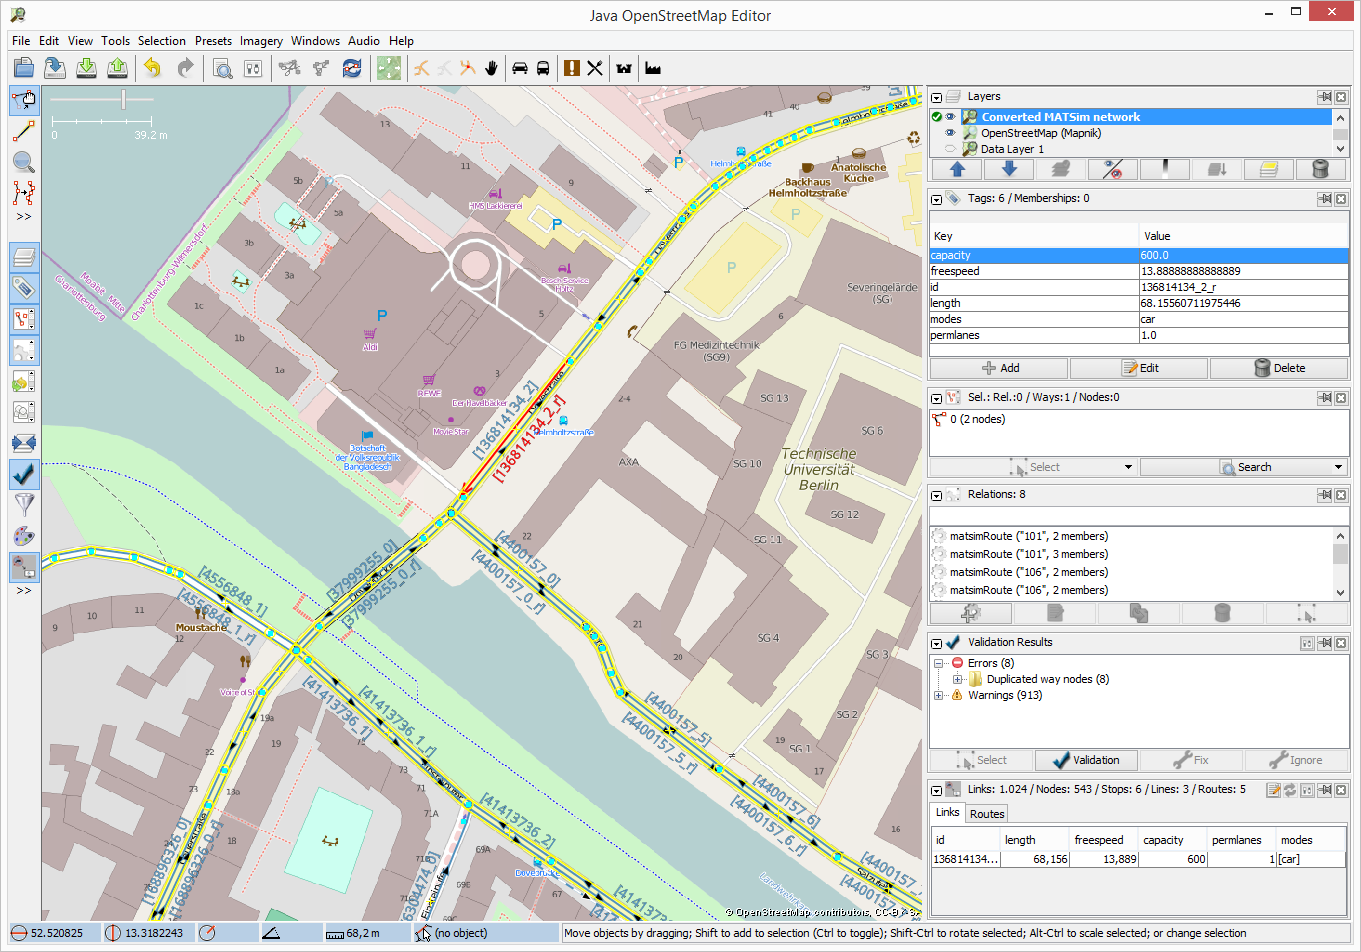
\includegraphics[width=0.4\textwidth, angle=0]{extending/figures/networkeditor/josm_screenshot} \end{center}

\kai{todo the below for the two editors.  See withinday planning for an example how to deal with two such sections}

% ##################################################################################################################
\section{Basic Information}
\label{sec:networkeditor-stdInfo}
% ============================================================================================
\subsection{MATSim JOSM Network Editor}
\label{sec:networkeditor-stdInfo1}
\createStandardInformationBasic{%
%
1
%
}{
%
2
%
}{
%
3
%
}{
%
4
%
}

% ============================================================================================
\subsection{networkEditorSingapore: Map-to-Map Matching Editors in Singapore}
\label{sec:networkeditor-stdInfo2}
\createStandardInformationBasic{%
%
\url{http://matsim.org/javadoc} $\to$ networkEditorSingapore
%
}{
%
\lstinline|gui.DoubleNetworkMatchingWindow| class, and \lstinline|gui.DoubleNetworkCapacitiesWindow| class
%
}{
%
in the GUI
%
}{
%
\citet[][]{Ordonez_Webpage_2011_3}
%
}

% ##################################################################################################################
\section{MATSim JOSM Network Editor}
A plugin for the \gls{josm} \citep[][]{JOSM2014}, is available, simplifying the process of creating and editing \gls{matsim} networks. This plugin fully integrates with \gls{josm}, benefiting from its built-in functionality.
%
% -------------------
\createfigure
{JOSM with converted MATSim network and \protect\gls{osm} background imagery}
{JOSM with converted MATSim network and \protect\gls{osm} background imagery. Map data taken from \citet[][]{OpenStreetMap2014}}
{\label{fig:networkeditor_screenshot}}
{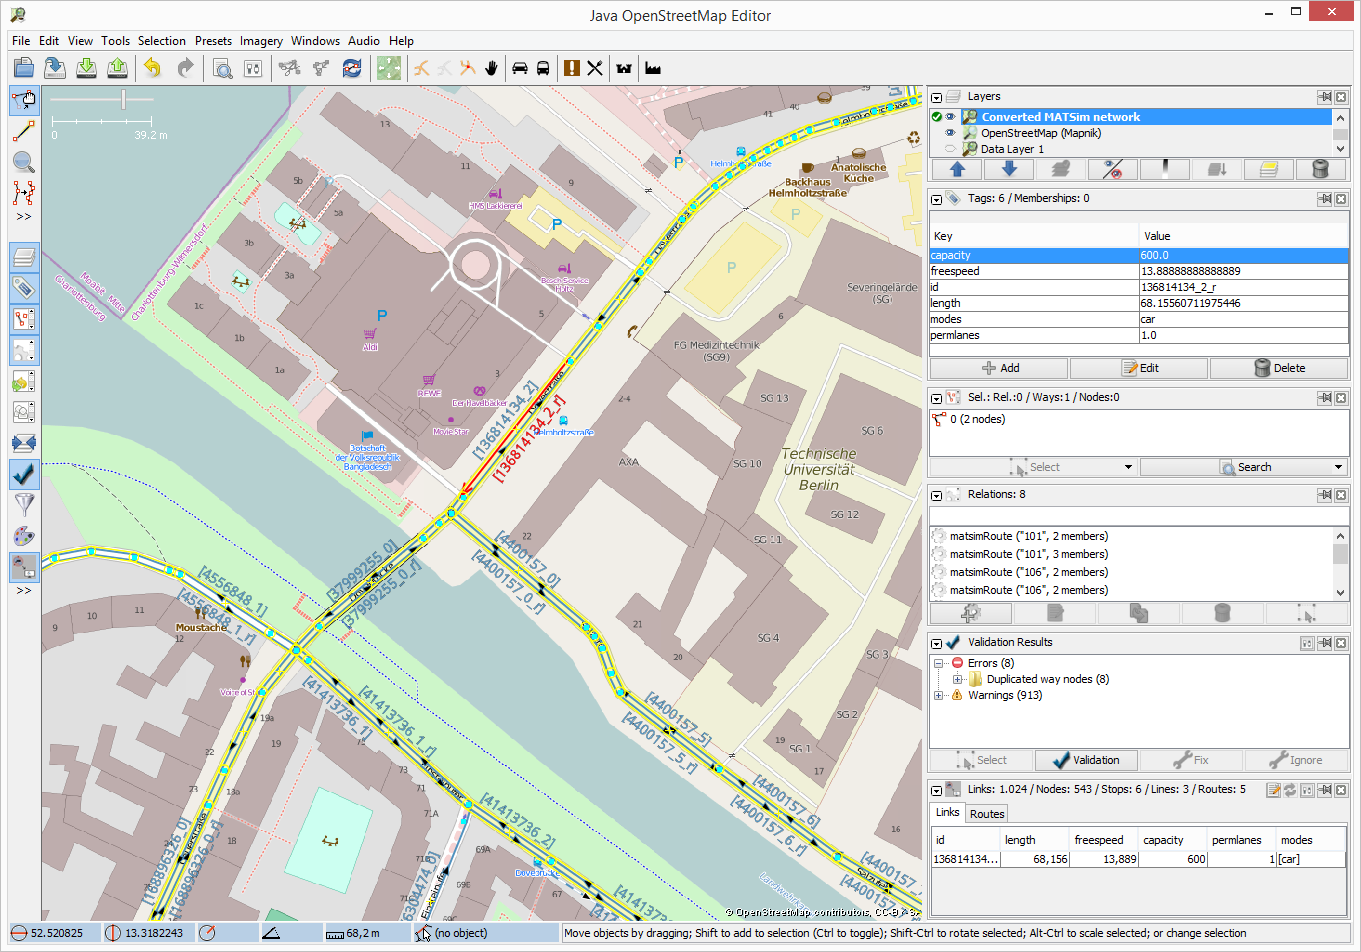
\includegraphics[width=1.0\textwidth]{extending/figures/networkeditor/josm_screenshot}}
{}
% -------------------

% ===========================================================================================
\subsection{Features}
The \gls{matsim} \gls{josm} lets a reader preview, edit and save a \gls{matsim} network directly from the map. Basic support for converting and editing public transport networks is implemented. The plug-in allows automatic post-processing of a network by removing unnecessary intermediate nodes and links.
\begin{description}\styleDescription
\item[Convert] \gls{matsim} networks from \gls{osm}. Load map data for a selected area directly from the Internet or load it from a local \gls{osm} file. Specify conversion parameters and save a \gls{matsim} network.
\item[Visualize] an existing or newly converted \gls{matsim} network along with other data like satellite imagery or other \gls{josm}-supported layers.
\item[Edit] an existing or newly converted \gls{matsim} network with the available \gls{josm} tools you know. Use the build-in undo and search functions of \gls{josm}. Changes to the underlying \gls{osm} data are immediately reflected by the converted \gls{matsim} network. Use \gls{matsim}-specific presets to minimize errors.
\item[Validate] an existing or newly converted \gls{matsim} network to comply with requirements of the \gls{matsim} network file description. Visualize errors and fix them (automatically). 
\end{description}
The next version will support public transport networks.

% ===========================================================================================
\subsection{Installing the Plug-In}
You do not need to download the source; it is in the \gls{josm} plug-in repository. Just start \gls{josm} and look for the \gls{matsim} plug-in under \lstinline|Edit...Preferences...Plugins|. Download the list of available plug-ins and search for ``matsim''. Tick the box, press \lstinline|ok| and restart \gls{josm}.

% ===========================================================================================
\subsection{Getting the Code}
The source code is hosted on github (\url{https://github.com/matsim-org/josm-matsim-plugin}). Unlike \gls{matsim}, the build is not based on \gls{maven}, but on Gradle. Editing the \lstinline|Manifest|, downloading \gls{josm} for compilation and building a flat \gls{jar} are easier in Gradle. Use your favorite \gls{ide} to import the Gradle project and/or see the comments in \lstinline|build.gradle| for details. You can run \gls{josm} and the plug-in in the debugger.
 
% ##################################################################################################################
\section{Map-to-Map Matching Editors in Singapore}
\label{sec:networkeditor-singapore}
For the Singapore scenario and supply data, a high resolution network was obtained from the \gls{navteq} company. This network consists of a graph representing every road in the island: very convenient for a high resolution model like \gls{matsim}. However, the information on travel capacities and network link free speeds is not accurate. To offset, local authorities provided the network model used for planning, which includes only major roads and simplified intersections, but capacities and free speed are accurately estimated. Figure~\ref{fig:Capacities} shows lower travel capacities of many primary roads in the navigation model (right), than in the planning model (left).

% -------------------
\createfigure
{Difference in the travel capacities}
{Difference in the travel capacities between the Singapore planning network model (left) and a navigation network model (right)}
{\label{fig:Capacities}}
{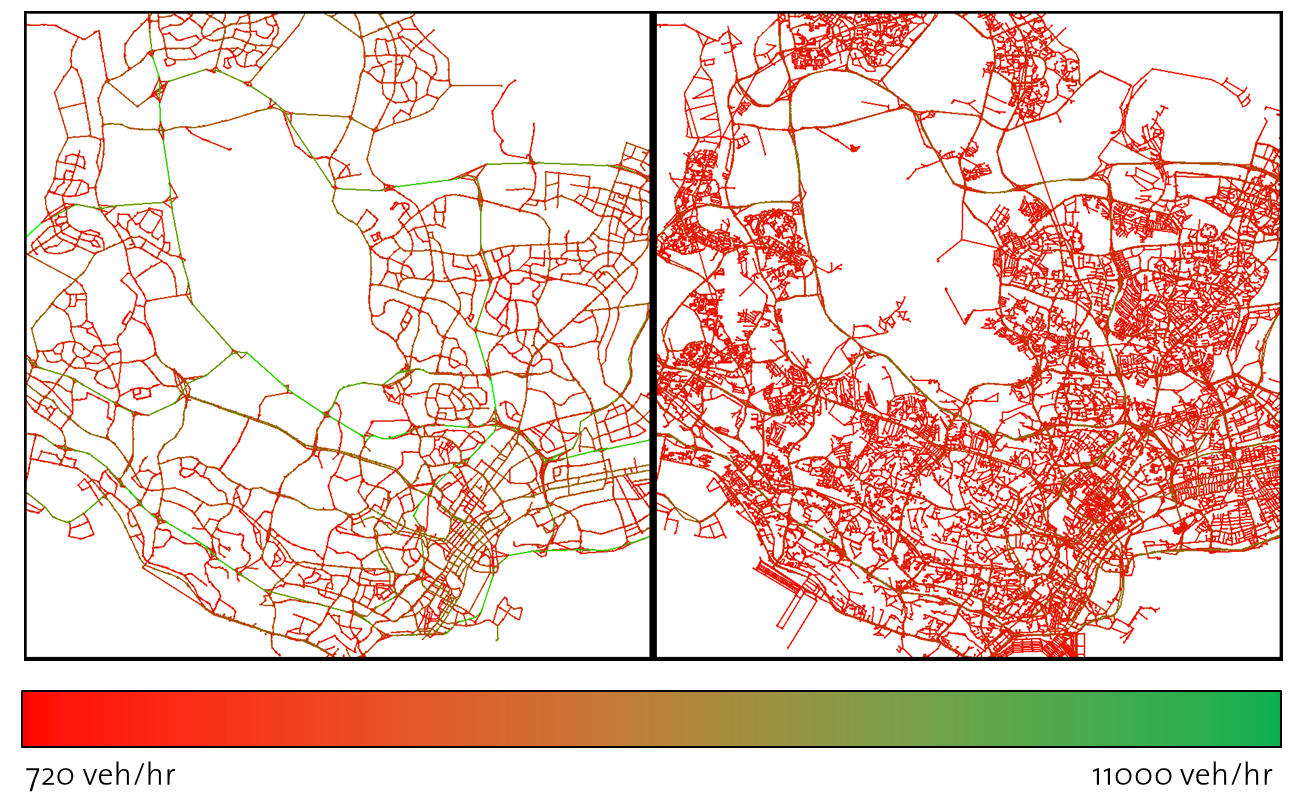
\includegraphics[width=1.0\textwidth]{extending/figures/netEdSing/Capacities.png}}
{}
% -------------------

This section describes a semi-automatic tool developed to match these two network models \citep[][]{Ordonez_Webpage_2011_3}, allowing updating of navigation network (high-res network) main links/capacities and free speeds with those of the planning network (low-res network).

% ===========================================================================================
\subsection{General Procedure}
Although many authors try to solve matching problems for two networks in a formal way, this work follows a semi-automatic approach. This means that automatic algorithms will be used to try and solve the problem, but the user knows the solution won't be perfect;  some manual work must be done. Hence, interactive tools are also provided to manually improve solutions.

The map-to-map procedure is based on the algorithm developed by \citet{BalmerEtAl_STRC_2005}. It consists of the following steps:
%
\begin{enumerate}\styleEnumerate
\item Classify nodes according to their topology (\eg source, sink, one way start, crossing) in both networks.
\item Reduce networks according to previous classification, and save relations to the original nodes.
\item Find crossings (set of close nodes) in both networks and relate them.
\item \textbf{Assuming not all crossings were found in the previous step, use the interactive tool shown in the Figure~\ref{fig:Nodes} to find all crossings in both networks and relate them}
\item Recognize links or sequences of links joining crossings found in (3) and (4)
\item \textbf{Assuming not all links or paths found in the previous step are correct, use the link-link matching interactive tool shown in the Figure~\ref{fig:Links}, to find or modify links or sequences of links joining the crossings}
\item Update capacities and free speeds of matched links found in (5) and (6)
\end{enumerate}
%
\createfigure
{Crossing-crossing matching application}
{Crossing-crossing matching application. A second node, matching the pink node on the (left) low-res network, is selected from the high-res network on the right}
{\label{fig:Nodes}}
{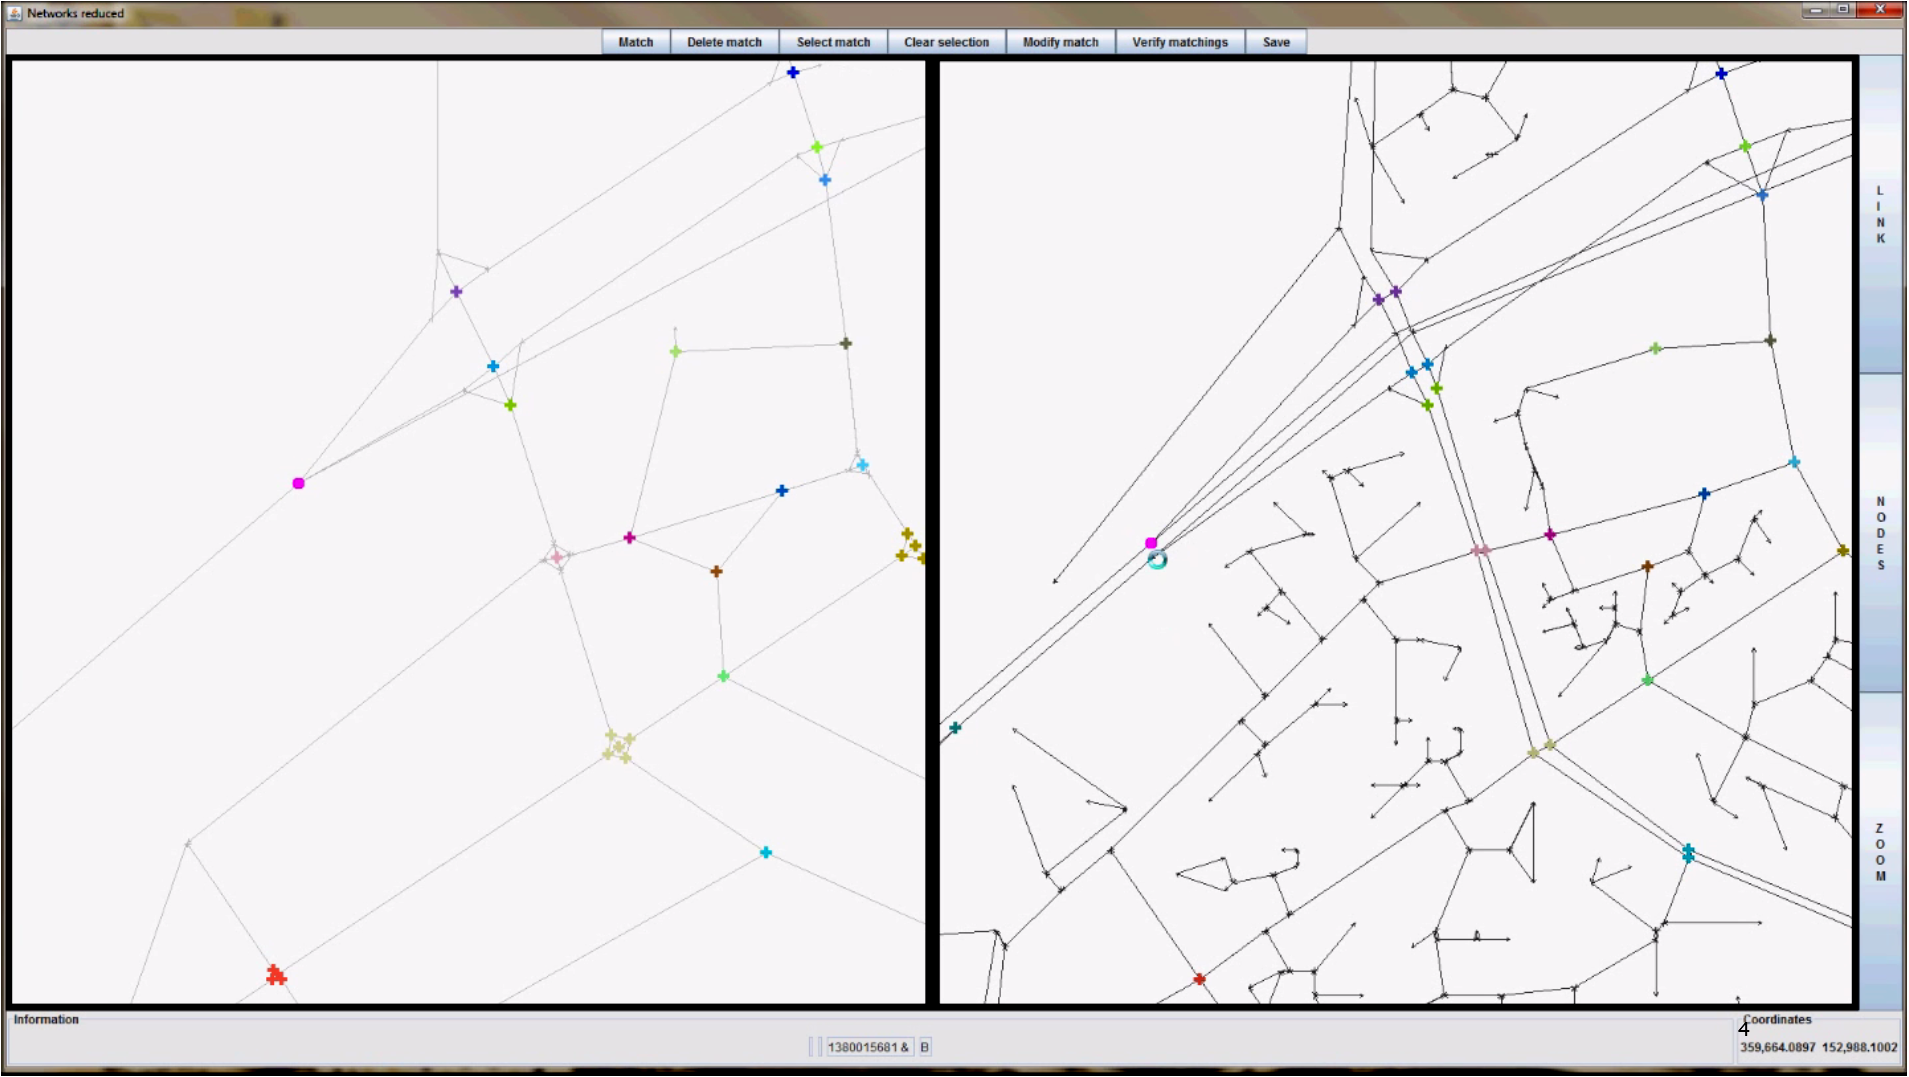
\includegraphics[width=1.0\textwidth]{extending/figures/netEdSing/Nodes.png}}
{}

% ===========================================================================================
\subsection{Interactive Tools Characteristics}
As shown in Figure~\ref{fig:Nodes}, the application allows interactive modifying of crossing-crossing relationships. A very similar interactive tool was also developed to modify link-link relationships between the high and low resolution networks. They can be found at the package \lstinline|playground.sergioo.networksMatcher2012|, in the playgrounds project of \gls{matsim}. To run the crossings-crossing application graphic interface, use the class \lstinline|gui.DoubleNetworkMatchingWindow|, and use the class \lstinline|gui.DoubleNetworkCapacitiesWindow| for the link-link application. These applications write simple text files of the relationships located. The program found at the class \lstinline|ApplyCapacities| overwrites capacities and/or free speeds, according to simple text files and writes the new resulting network \gls{xml} file. This multiple-steps design enables running interactive applications several times, or in parallel. The interactive tools' developed functional requirements and quality attributes are:
%
\createfigure
{Link-link matching application}
{Link-link matching application. A shortest path algorithm to select a sequence of right-hand network links will be executed when clicking the destination node}
{\label{fig:Links}}
{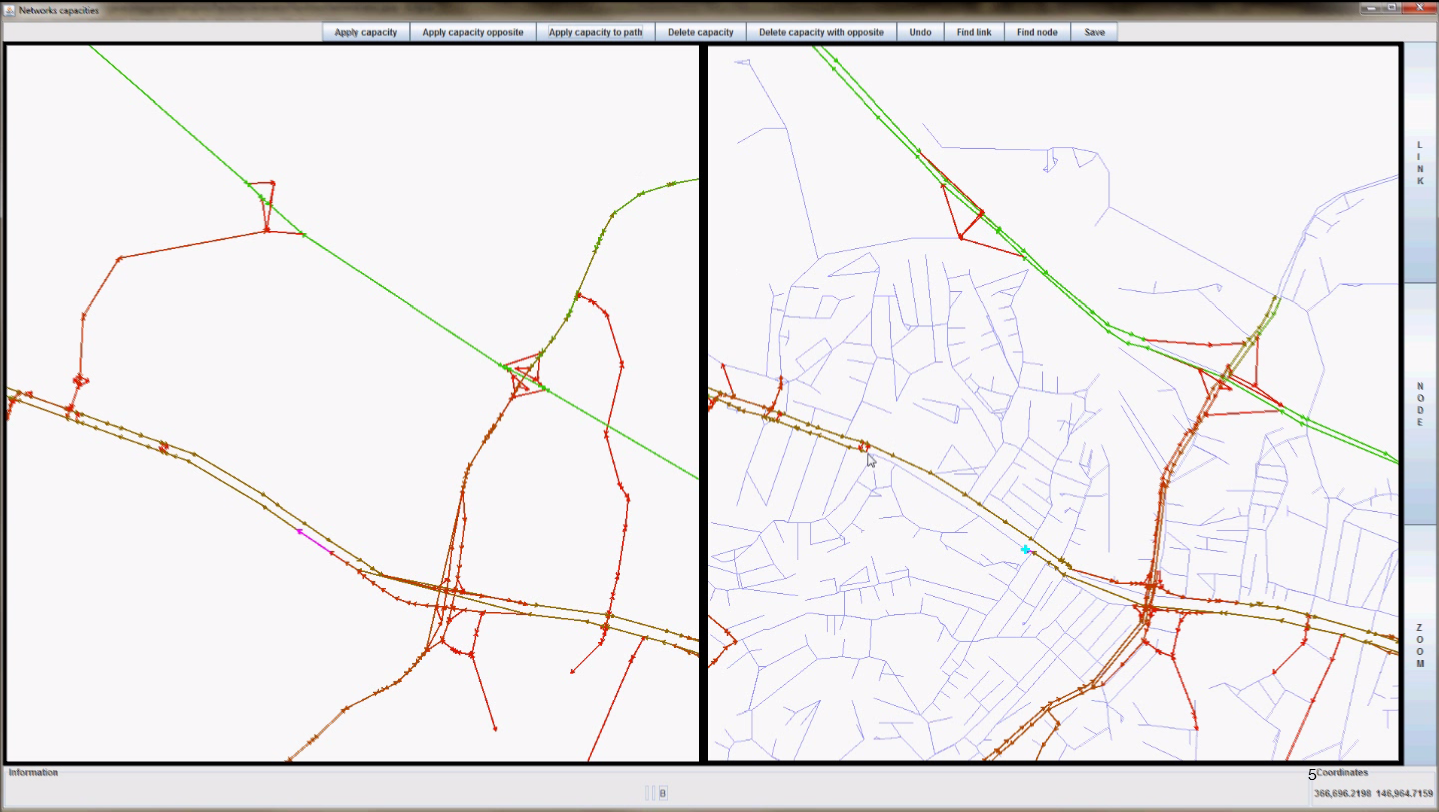
\includegraphics[width=1.0\textwidth]{extending/figures/netEdSing/Links.png}}
{}

\begin{itemize}\styleItemize
\item Visualization: Two navigation networks are displayed in two modes. The first mode splits the window in two, showing each network on one side and maintaining them at the same geographical position and zoom when navigating. The second superimposes both networks in the same window, with only one active. Selected elements are drawn in different colors. Everything is displayed in a bi-dimensional interactive way, showing the cursor location in the working coordinates and including panning, zoom and view-all options. The crossing-crossing application displays matched sets of nodes (crossings), with the same color in both networks. The link-link application tool also allows visualization of the capacity (or free speed) property value of both networks' links, using a color scale, as shown in Figure~\ref{fig:Links}.
\item Selection: The applications enable selection of links and nodes from both networks. The crossing-crossing option allows only selection of node sets. The link-link application allows selection of links' sequence. This can be done directly, or by selecting an origin node, a destination node and running a ``select shortest path algorithm tool''. It is also possible to select the other link instead of the first one chosen.
\item Matching and Deletion: The applications allow creation of a similarity relationship between elements selected in both networks, sets of nodes, or sequences of links.
\item Saving: The applications allow located relationships to be saved.
\item Loading: The applications allow the loading of previously located relationships.
\item Others: The crossing-crossing application executes and automatically verifies currently found matching, to avoid repeated nodes. It also enables clearing of the current selection. The link-link application allows automatic navigation to a link, or node, specified by the user, using its ID. It also enables the undoing of previous matching. 
\end{itemize}

% ===========================================================================================
\subsection{Results}
All low-res network links were matched to high-res links, updating the corresponding link properties. Figure~\ref{fig:Results} shows the differences in travel capacities between original navigation network values and the final version. Eight hours of manual work were required to match crossings and ten hours of manual work to match links. Obviously, improvements in accuracy and completeness of the automatic matching algorithms reduce the manual work time.
%
\createfigure
{Resulting changes in navigation network travel capacity property}
{Resulting changes in navigation network travel capacity property}
{\label{fig:Results}}
{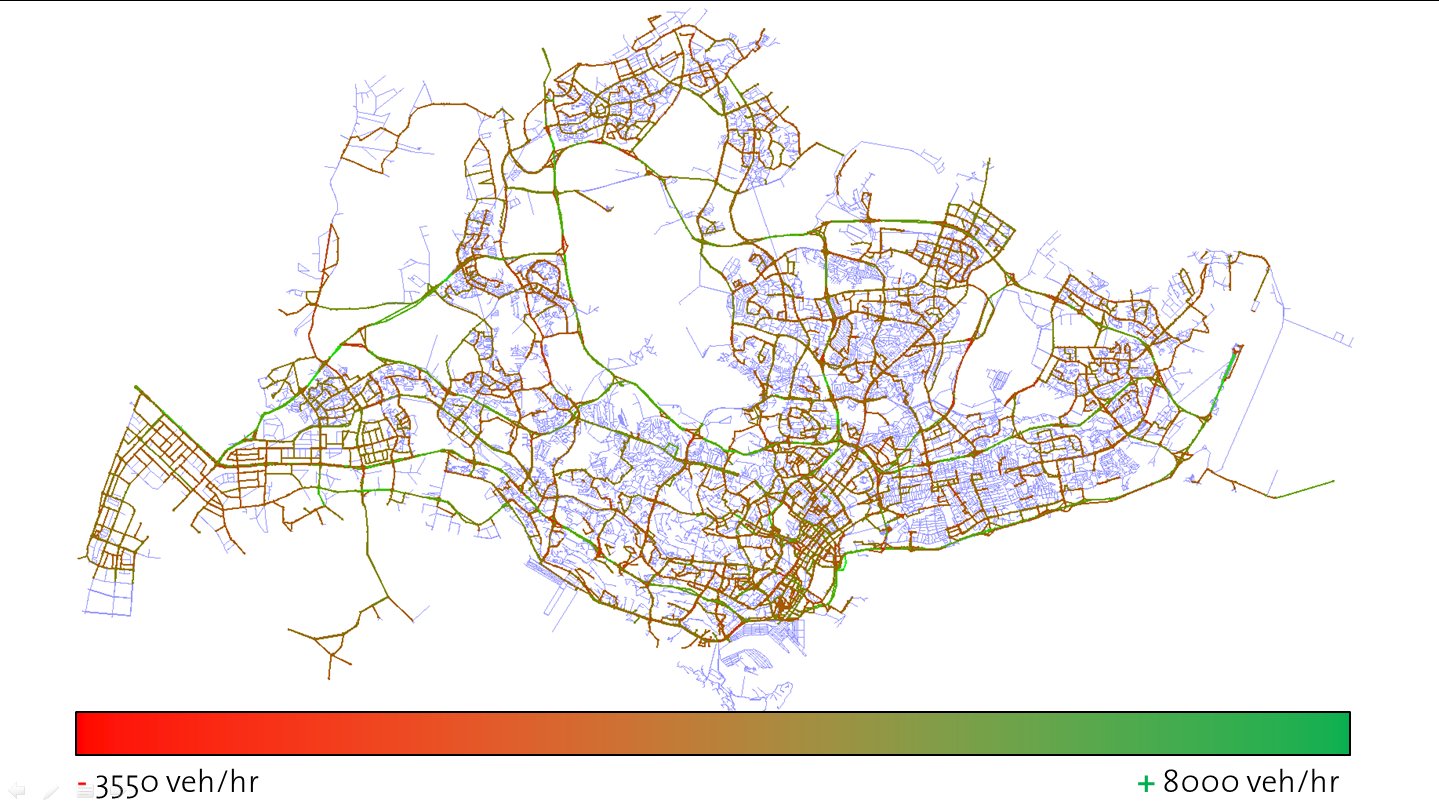
\includegraphics[width=1.0\textwidth]{extending/figures/netEdSing/Result.png}}
{}

% ##################################################################################################################
